\begin{center}
  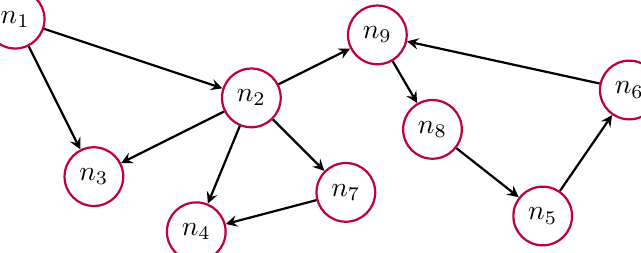
\begin{tikzpicture}[remember picture]
    \tikzstyle{edge}  = [thick,>=stealth,draw=black]
    \tikzstyle{dedge} = [thick,->,>=stealth,draw=black]
    \tikzstyle{node}=[
      overlay,
      circle,
      draw=purple,
      anchor=center,
      thick,
      minimum size=1,
    ]
    
    \node[node] (n1) at (-4,0) {$n_1$};
    \node[node] (n2) at (-1,-1) {$n_2$};
    \node[node] (n3) at (-3,-2) {$n_3$};
    \node[node] (n4) at (-1.7,-2.7) {$n_4$};
    \node[node] (n5) at (2.7,-2.5) {$n_5$};
    \node[node] (n6) at (3.8,-0.9) {$n_6$};
    \node[node] (n7) at (0.2,-2.2) {$n_7$};
    \node[node] (n8) at (1.3,-1.4) {$n_8$};
    \node[node] (n9) at (0.6,-0.2) {$n_9$};
    
    \draw[dedge] (n1)--(n2);
    \draw[dedge] (n2)--(n3);
    \draw[dedge] (n1)--(n3);
    \draw[dedge] (n2)--(n4);
    \draw[dedge] (n2)--(n9);
    \draw[dedge] (n9)--(n8);
    \draw[dedge] (n6)--(n9);
    \draw[dedge] (n5)--(n6);
    \draw[dedge] (n2)--(n7);
    \draw[dedge] (n7)--(n4);
    \draw[dedge] (n8)--(n5);
  \end{tikzpicture}
\end{center}
